\section{Avbrudd}
\label{sec:avbrudd}

\emph{Eksterne avbrytelser} refererer til situasjoner hvor en ekstern hendelse fører til en forstyrrelse i prosessen med å fullføre en oppgave \citep{Harr07}.

\subsection{Dualiteten ved avbrudd}
\citet{Grundgeiger09} skiller mellom \emph{gode} og \emph{dårlige} avbrudd, og hevder disse må sees i sammenheng med hvilke effekter de har. Eksempler på positive effekter er øyeblikkelig kommunikasjon og tilgang til viktig informasjon. Avbryter opplever å få en umiddelbar bekreftelse på at informasjonen er mottatt og kan dermed avlaste arbeidsminnet, mens den som blir avbrutt kan oppleve negative effekter, som overbelastet kognitiv kapasitet, forsinkelse i eget arbeid, stress og frustrasjon. Samtidig kan avbruddet ha en positiv effekt dersom den avbrutte mottar ønsket informasjon.


\subsection{Avbruddshåndtering}
Gitt denne dualiteten kan avbruddshåndtering sies å ha to mål: (1) redusere de negative effektene, og (2) utnytte de positive effektene ved avbrudd. \citet{Grandhi10} gir fire teknikker for avbruddshåndtering:
\begin{enumerate}        
\item Forebygging - bruk av funksjoner som forebygger eller blokkerer innkommende avbrytelser. Dette kan gjøres enkelt ved å for eksempel skru av mobilen for en periode. En annen strategi er å kontrollere timingen til avbruddet, eller å kun tillate avbrytelser som er relevant for den oppgaven man utfører. Dette krever at awareness-informasjon er tilgjengelig, slik at timingen kan justeres for å minske den negative effekten ved avbruddet.

\item Fraråding - bruk av funksjoner som fraråder avbrytelser. Dette skjer ofte ved at man gir informasjon til avbryter om tilgjengeligheten til den man ønsker å avbryte. 

\item Modifiserte varslinger - bruk av funksjoner som modifiserer hvordan individer varsles om innkommende anrop. Ved bruk av ulike modaliteter som lyd, vibrasjon og lys, kan man minimere interferensen mellom perseptuelle og kognitive prosesser involvert i avbruddshåndtering og oppgaveytelse \citep{Harr07}.

\item Forhåndsvisning - bruk av funksjoner som gir informasjon om selve avbrytelsen som den avbrutte selv kan reflektere over.   
\end{enumerate}

\noindent
\citet{Harr07} presenterer fler aspekter knyttet til sosial kontekst, blandt annet lokasjonsbasert forstyrrelse og indirekte forstyrrelse.

\noindent
Avbrudd kan ha effekter på andre mennesker som befinner seg på samme lokasjon som den som blir avbrutt. Dette illustreres i figur \ref{collateral}, hvor interaksjonen mellom aktør D (avbryter) og aktør B (den som avbrytes) også påvirker aktører A og C.
\begin{figure}[H]
\centering
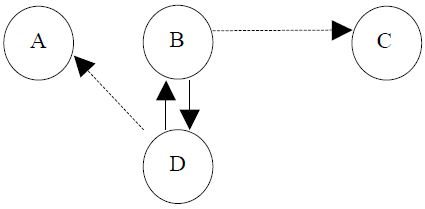
\includegraphics[scale=0.5]{collateral.jpg}
\caption{Lokasjonsbasert forstyrrelse}
\label{collateral}
\end{figure}

\noindent
Aktører B og C må ikke nødvendigvis kommunisere direkte, men aktør C kan være avhengig av tiden, innholdet og kvaliteten aktør Bs oppgave resulterer i. Dermed kan en forstyrrelse av aktør B også indirekte forstyrre aktør C.

\begin{figure}[H]
\centering
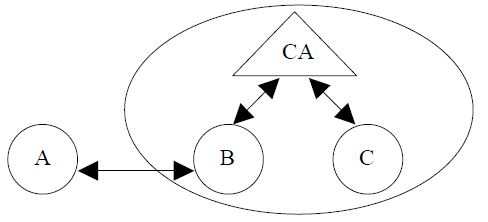
\includegraphics[scale=0.5]{dropball.jpg}
\caption{Samarbeid og avbrudd - indirekte forstyrrelse}
\label{indirekte}
\end{figure}

\subsection{Utfordringer}
\citet{Harr07} påpeker tre fundamentale utfordringer ved avbruddshåndtering: (1) fare for å miste informasjon, (2) mindre privatliv og (3) utsettelse av oppgaver. For hver situasjon må individer finne den optimale balansen mellom isolasjon og tilgjengelighet, åpenhet og privatliv, og direkte eller utsatt håndtering av avbruddene.